\documentclass[tikz]{standalone}
\usepackage{tikz}
\usetikzlibrary{arrows.meta,positioning,shapes.geometric,shapes.misc,fit,backgrounds,calc,decorations.pathreplacing}

\definecolor{cProposer}{HTML}{2B7A78}
\definecolor{cBuilder}{HTML}{3D5A80}
\definecolor{cDocumenter}{HTML}{C07C38}
\definecolor{cVerifier}{HTML}{A04050}
\definecolor{cCoordinator}{HTML}{6B5CA5}
\definecolor{cMonitor}{HTML}{488B49}
\definecolor{cBottleneck}{HTML}{A04050}

\begin{document}
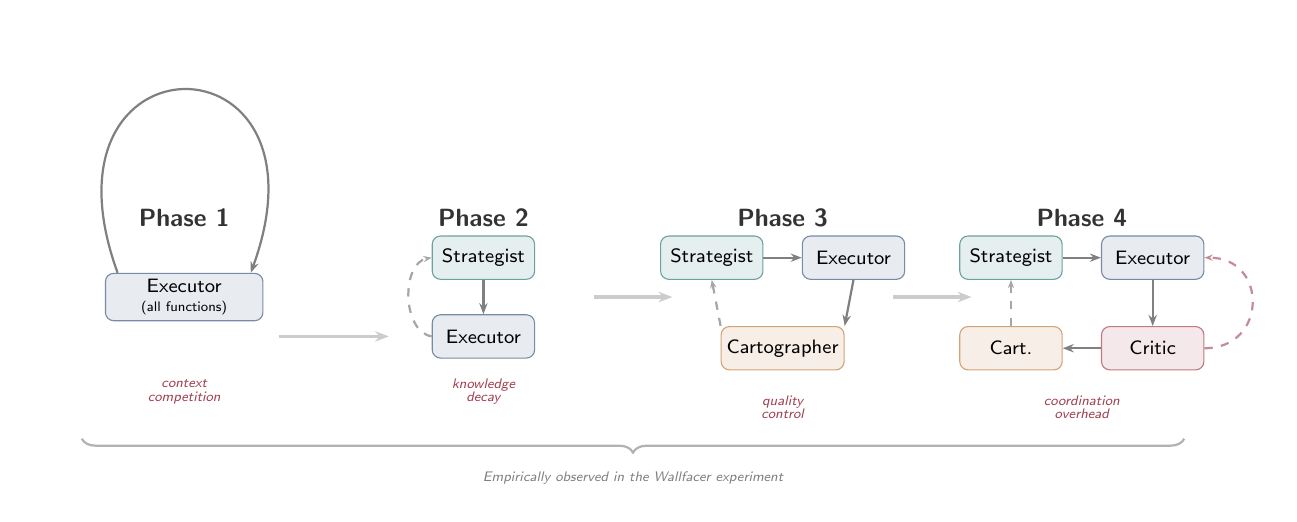
\begin{tikzpicture}[
    agent/.style={rectangle, rounded corners=3pt, draw=#1!70, fill=#1!12, minimum width=1.3cm, minimum height=0.55cm, font=\scriptsize\sffamily, inner sep=2pt, align=center},
    agent/.default={cBuilder},
    phase/.style={font=\small\sffamily\bfseries, text=black!80},
    bottleneck/.style={font=\tiny\sffamily\itshape, text=cBottleneck, align=center},
    arr/.style={-{Stealth[length=4pt]}, thick, black!50},
    farr/.style={-{Stealth[length=3pt]}, thick, dashed, black!35},
    trans/.style={-{Stealth[length=5pt]}, very thick, black!20},
]

\def\sep{3.8}

% Phase 1
\node[phase] at (0, 2.5) {Phase 1};
\node[agent=cBuilder, minimum width=2cm] (b1) at (0, 1.5) {Executor\\[-1pt]{\tiny(all functions)}};
\draw[arr, looseness=5] (b1.160) to[out=110,in=70] (b1.20);
\node[bottleneck] at (0, 0.3) {context\\[-1pt]competition};

\draw[trans] (1.2, 1.0) -- (\sep-1.2, 1.0);

% Phase 2
\node[phase] at (\sep, 2.5) {Phase 2};
\node[agent=cProposer] (p2) at (\sep, 2.0) {Strategist};
\node[agent=cBuilder] (b2) at (\sep, 1.0) {Executor};
\draw[arr] (p2.south) -- (b2.north);
\draw[farr] (b2.west) to[out=170,in=190] (p2.west);
\node[bottleneck] at (\sep, 0.3) {knowledge\\[-1pt]decay};

\draw[trans] (\sep+1.4, 1.5) -- (2*\sep-1.4, 1.5);

% Phase 3
\node[phase] at (2*\sep, 2.5) {Phase 3};
\node[agent=cProposer] (p3) at (2*\sep-0.9, 2.0) {Strategist};
\node[agent=cBuilder] (b3) at (2*\sep+0.9, 2.0) {Executor};
\node[agent=cDocumenter] (d3) at (2*\sep, 0.85) {Cartographer};
\draw[arr] (p3) -- (b3);
\draw[arr] (b3.south) -- (d3.north east);
\draw[farr] (d3.north west) -- (p3.south);
\node[bottleneck] at (2*\sep, 0.1) {quality\\[-1pt]control};

\draw[trans] (2*\sep+1.4, 1.5) -- (3*\sep-1.4, 1.5);

% Phase 4
\node[phase] at (3*\sep, 2.5) {Phase 4};
\node[agent=cProposer] (p4) at (3*\sep-0.9, 2.0) {Strategist};
\node[agent=cBuilder] (b4) at (3*\sep+0.9, 2.0) {Executor};
\node[agent=cDocumenter] (d4) at (3*\sep-0.9, 0.85) {Cart.};
\node[agent=cVerifier] (v4) at (3*\sep+0.9, 0.85) {Critic};
\draw[arr] (p4) -- (b4);
\draw[arr] (b4.south) -- (v4.north);
\draw[arr] (v4) -- (d4);
\draw[farr] (d4.north) -- (p4.south);
\draw[farr, cVerifier!60] (v4.east) to[out=0,in=0,looseness=1.8] (b4.east);
\node[bottleneck] at (3*\sep, 0.1) {coordination\\[-1pt]overhead};

% Bottom annotation
\draw[decorate, decoration={brace, amplitude=5pt, mirror}, thick, black!30] (-1.3, -0.3) -- (3*\sep+1.3, -0.3);
\node[font=\tiny\sffamily\itshape, text=black!50] at (1.5*\sep, -0.8) {Empirically observed in the Wallfacer experiment};

\end{tikzpicture}
\end{document}
